\documentclass[preprint]{elsarticle}
\biboptions{round, numbers}
\usepackage[latin1]{inputenc}
%\usepackage[T1]{fontenc}
%\usepackage{textcomp}
\usepackage{graphicx}
\usepackage{color}
%\usepackage{setspace}
\usepackage{url}
\usepackage[english]{babel}

\begin{document}

\begin{frontmatter}

%%%%%%%%%%%%%%%%%%%%%%%%%%%%%%%   TITLE   %%%%%%%%%%%%%%%%%%%%%%%%%%%%%%%

\title{A Review on Corporate Security Solutions. A Comparison with a User-Centric and Self-Adapted System}

%%%%%%%%%%%%%%%%%%%%%%%%%%%%%%%   AUTHORS   %%%%%%%%%%%%%%%%%%%%%%%%%%%%%%%

\author{P. de las Cuevas, A.M. Mora, J.J. Merelo}
\ead{\{paloma, amorag, jmerelo\}@geneura.ugr.es}
\address{Departamento de Arquitectura y Tecnolog�a de Computadores.\\ ETSIIT - CITIC. University of Granada, Spain}
%\author{A. M. Mora}
%\ead{amorag@geneura.ugr.es}
%\address{Departamento de Arquitectura y Tecnolog�a de Computadores. Escuela T�cnica Superior de Ingenier�as Inform�tica y de Telecomunicaci�n. CITIC. University of Granada, Spain}

%\maketitle

%
%%%%%%%%%%%%%%%%%%%%%%%%%%%%%%%%%   ABSTRACT   %%%%%%%%%%%%%%%%%%%%%%%%%%%%%%%%%
%
\begin{abstract} 
Enterprises, and their Chief Security Officers (CSOs) particularly, want to be sure that their Security Policies are complied. This goal turned hard to achieve since employees are able to use their own devices (laptops, smartphones, and tablets) at work, or at home but for work purposes. As this is part of the Bring Your Own Device (BYOD) philosophy and is being adopted by many companies everyday, a number of solutions have arisen in order to adapt it securely. In this paper, the most relevant solutions are presented, and so is displayed the European MUSES (Multiplatform Usable Endpoint Security) project, which tries to go further this state of the art, taking into account user behaviour for security rules adaption.
\end{abstract}

%
%%%%%%%%%%%%%%%%%%%%%%%%%%%%%%%%%   KEYWORDS   %%%%%%%%%%%%%%%%%%%%%%%%%%%%%%%%%
%
\begin{keyword}
BYOD \sep Corporate mobile security \sep End-to-end security solutions \sep User-centric systems \sep Self-adaptation \sep Multiplatform \sep Information Asset \sep Security Policies \sep Data security and data privacy.
\end{keyword}

\end{frontmatter}


%-------------------------------------------------------------------------------
%%%%%%%%%%%%%%%%%%%%%%%%%%%%%%%   INTRODUCTION   %%%%%%%%%%%%%%%%%%%%%%%%%%%%%%%
%-------------------------------------------------------------------------------

\section{Introduction}
\label{sec:intro}

Some years ago, company data were stored in owned servers which were accessed by the employees or users by means of desktop or portable computers. Nowadays it is frequent that these data are distributed among multiple machines, even not all belonging to the company and working over the famous Cloud Computing environment. Besides, being stored in the cloud or not, data is being consulted and modified through a wide amount of devices, some of them owned by the company's users. This is the so-called Bring Your Own Device (BYOD) philosophy. It is becoming highly successful due to the impact that smartphones and tablets are having in the market.
Data security and privacy are key factors for a company, thus, to protect them, it is usual to define Organisational Security Policies. Their definition is nowadays a very difficult problem, since the BYOD tendency means that several factors must be considered \cite{Opp_Security11}, most of them previously ignored or non considered in security systems, for instance the current mixture between personal and professional information in these devices (the user could navigate inside social networks where there could be friends and also company partners or clients).

Moreover, it has been demonstrated that people are the main hazard regarding the company security \cite{Adams_Users05}, so in this situation, some monitorization and security-aimed applications are arising, aiming to cope with the concept of seamless working experience on different devices. 
This concept is a methodology of work which allows users to start/continue a working session over multiple devices and locations without any significant loss of data. This new situation has a big impact from the point of view of the security \cite{Schu_SecPatterns05}, since the company's data borders have changed in the last years so now the users can access significant data from outside the enterprise, and possibly through a non absolutely secure channel.

In this scenario several solutions have arisen in order to manage the corporate security. Most of them try to be non-intrusive (regarding the users' personal data), friendly and easy to use. This paper presents an overview of the main solutions, describing their features, and introduces a novel (still in development) system named MUSES, from Multiplatform Usable Endpoint Security. In addition, the paper compares those main solutions with MUSES, which is being implemented inside an European project and will provide a device independent, user-centric, and self-adaptive corporate security system, to deal with the aforementioned seamless working.
MUSES will analyse the users' behaviour and predict, using computational intelligence methods, risky or dangerous actions regarding both an event correlation and a risk and trust analysis engines. The system will be able to learn from the user's past behaviour, and react, in a non-intrusive way, to the potentially dangerous sequence of actions that he or she is conducting at any time.

The rest of the paper is organized as follows. First, some background situation about enterprise security is presented in Section \ref{sec:preliminaryconcepts}, explaining how BYOD affects it. Then, some solutions from different companies are detailed in Section \ref{sec:toolsreview}, being specified for each one if the correspondent tool is available or, if not, the approximate release date. Some solutions are focused only in smartphones, while others are thought for laptops; also some are implemented for a certain platform, but others consider multiplatform. 
Then, in Section \ref{sec:muses}, the Multiplatform Endpoint Security System is presented. Its advantages and benefits in comparison with the other solutions are commented in Section \ref{sec:comparison}.
Finally, the conclusions are discussed in Section \ref{sec:conclusions}.


%----------------------------------------------------------------------------
%%%%%%%%%%%%%%%%%%%%%%%%%%%%%%%   BACKGROUND  %%%%%%%%%%%%%%%%%%%%%%%%%%%%%%%
%----------------------------------------------------------------------------


\section{Preliminary concepts and background about enterprise security}
\label{sec:preliminaryconcepts}

Until these days, enterprises used to follow a static Security Policy devoted to controlling a certain structure \cite{BYOD13}, where the Information Assets and the devices were purchased and maintained by the company. Now that corporate networks are becoming dynamic for being adapted to the BYOD philosophy, there is an additional risk because the devices that the employees use are not always company-owned. A needed security policy, or in this case, an Information Security Policy (ISP from now on) should deal with the way of protecting a certain organization's information against a security breach. Though there are standards, such as ISO27002 or Security Forum's Standard of Good Practice\footnote{https://www.securityforum.org}, and many guidelines \cite{SecPol09}, an ISP is built depending on the characteristics of the community/organisation that they are built for.

On the other hand, employee-owned devices like smartphones, they are not just for work purposes anymore. As the name says, smartphones are more than simple old cell phones, and people who use them in their works have the possibility of maintaining a good balance between work and private life. For this reason, the risk of uncontrolled devices accessing to corporate access in unsafe conditions, due to the number of risky applications, is bigger.

Normally, enterprise network architecture was being adapted to cope with external attackers \cite{MIT05}. With the incorporation of BYOD, the threat is about corporate assets being compromised due to employees' devices with vulnerabilities \cite{android11}, or leaked because they are being accessed from a device connected through an unsecure (public) network.

Thus now, more things should be considered than the usual ones when designing a company's network architecture. In Figure \ref{fig:proposed_diagram} there is a proposal which can be used for the beginning of the study of solutions that may secure such a dynamic environment. It includes the possibility of having employee-owned mobile (smartphones and tablets) and portable (laptops) devices, and also the opportunity that the employees have of connecting these devices either from inside or outside the company premises. Moreover, company's information assets are constantly accessed under these conditions, considering that an information asset means every \textit{piece of information} that has a \textit{value} (cost depending on the risk of being lost or leaked) for the company, and that can be from files with sensitive information to certain mails, or even company applications.

The other issue to cope with is the elaboration of a good ISP, understandable for every user of the company, and more importantly, non intrusive for them. A lot of researchers have studied the natural tendency of employees to comply with the ISP \cite{SecPolComp07,SecPolComp10,SecPolComp12}, reaching conclusions such as the employees compliance with the security policies increases educating/training them in information security awareness  \cite{SecPolComp09}, and decreases applying too much sanctions when a misuse or abuse occurs \cite{SecPolPenalty09}. For each tool in Section \ref{sec:toolsreview} it is specified if the developers have taken into account the construction of ISPs, or even if they give some guidelines for building them.

This situation leads to a need of protecting the organisation's side, but also the users' side, making non-interfering easy-to-follow ISPs and leaving them to use their devices for personal purposes while working whithout putting organisation's information assets under risk. The compliance of these requirement would compose an End-to-End Security Solution (protecting both enterprise and employee), which is the motivation for the development of the tools reviewed and, as presented in Section \ref{sec:muses}, is the aim of the MUSES project.

\begin{figure}
	\begin{center}
		\includegraphics[scale=0.4]{img/proposed_diagram.eps}
		\caption{Architecture approach of an Enterprise Network assuming that the Company has adopted the BYOD philosophy.}
	\label{fig:proposed_diagram}
	\end{center}
\end{figure}

%------------------------------------------------------------------------------
%%%%%%%%%%%%%%%%%%%%%%%%%%%%%%%   TOOLS REVIEW  %%%%%%%%%%%%%%%%%%%%%%%%%%%%%%%
%------------------------------------------------------------------------------

\section{Tools for corporate mobile security}
\label{sec:toolsreview}

Now that BYOD philosophy is becoming a tendency, a number of tools appeared by now, and others are under development but expected to be released soon. They were specifically designed for CSOs and Chief Information Security Officers (CISOs) to secure, monitor, and act over spartphones and other personal mobile or portable devices, when they become too risky. Some of those tools have influenced the development of the MUSES European project itself, showed in Section \ref{sec:muses}. The present section explains the mentioned products that can be considered related to MUSES objectives.

% Don't completely like the intro for being too focused to MUSES.

%----------------------------------------------------------------------------

\subsection{IBM Hosted Mobile Device Security Management}
\label{subsec:ibm}

One of the first companies who supported the BYOD model was IBM in 2011 \cite{IBM_tool}, as they recognized the increase of employees who brang their personal smartphones or tablets into the workplace. To help organizations \cite{ibm11} embrace both company and employee owned mobile devices (as said, this practise is part of the BYOD model) in a security-rich environment, IBM developed a mobile device security management solution. For IBM, a mobile security strategy should focus on several key areas.

On the one hand, the organization should identify which business data the strategy will allow to be stored and processed on which mobile devices. This helps determine what needs to be protected and to what degree. Then, because different mobile platforms have different native security mechanisms, the organization needs to define which mobile device platforms will be allowed in the business environment and, thus, need to be supported in the mobile security strategy and plan. That means, to define the scope of the security plan. Also there is need to decide the responsibility for mobile security management work, whether using the current IT security team to handle mobile devices, or outsourcing to a managed security service provider. And no matter what the mobile environments, a number of mobile ISPs and best-practise procedures need to be put in place and should also be identified in the company's mobile security strategic plan.

Taking into account these considerations, IBM developed a framework that specifies security domains and levels for applying various security technologies. When applied to mobile devices (not portable ones, so that laptops are not considered), the features of this framework depend on the deployment:

\begin{description}
	\item[Identity and access] Not only the use of strong passwords when accesing the devices, but also supply two way authentication and VPN access control, by supervising the authorised IP addresses and adding re-authentication for accessing resources (assets) with high value.
	\item[Data protection] Data security stored in the devices, related to profesional life, is encrypted, also during the transmission. Moreover, when a device is lost, data can be removed remotely, and the device located or locked out (locking out a device is also made after a modifiable timeout). Finally, back ups are performed periodically once the device has been recovered.
	\item[Application security] This is related to the requirement of being connected from a controlled location for authorising the download of business applications, and those applications must be certified (also the currently running on the device). Actually, IBM's tool can monitor and remove applications which are identified as untrustwothy or unsafe.
	\item[Fundamental integrity control] Running both antimalware software and personal firewall, and making the result of these tests as dependency for VPN's intranet access. 
	\item[Governance and compliance] Taking into consideration the mobile security as an important point in the overall risk management program of the company, and extend the periodic security audits to mobile devices too.
\end{description}

The considered architecture for this solution is a client-server architecture, where the controlling center is placed in the server, and the client would be installed on the mobile devices. This way, the client/device would communicate with the server as regularly as possible, to enforce policies, execute commands, and report status. With these features, and by analysing in the server the incoming data from the devices, this IBM's solution would be able to help enterprises to support ISPs compliance and to recognise (consequently acting over) mobile threat landscapes.

%Regarding IBM hosted mobile device security solution's architecture, the solution is built on a sound client-server architecture in which the server centrally controls and manages security policies and settings for various security features. The client would be installed on the mobile device and regularly communicate with the server to enforce policies, execute commands and report status. Also, IBM's solution contains reporting and analysis capabilities, with information that helps the company to support ISP compliance, recognize the mobile threat landscape and evaluate the solution's effectiveness in countering threats.

%----------------------------------------------------------------------------

\subsection{Sophos Mobile Control}
\label{subsec:sophos}

Sophos is a company founded in 1985 focused on IT security and data protection for businesses. Their \textit{Mobile Device Management} main product \cite{Sophos_tool} is Sophos Mobile Control. It is oriented to IT administration for mobile devices, trying to offer to the users the possibility of choosing the delivery model to suit their needs, i.e., between on-premise and Software as a Service (SaaS).

The tool offers the possibility of managing all workers and co-workers smartphones and tablets from a single-based console. The console monitors the devices throughout their full lifecycle: from the initial set up and enrolment, right through to decommissioning. Other features are similar to IBM's product, adding some new like being able to connect to an existing user directory using Lightweight Directory Access Control (LDAP)\footnote{LDAP is an application protocol for accessing and maintaining distributed directory information services over an Internet Protocol (IP) network.}.
	
Additional security is provided by the incorporation of \textit{Malware and Web protection}, so that the user does not need to install anti-malware software by him or herself. Regarding compliance enforcement, the main goal is not to sacrifice company's security in favour of flexibility for the users, which has been demonstrated \cite{SecPolPenalty09} that could result in bad (unwilling or not) users' beviour. Thus, company's BYOD initiative should include an acceptable use policy to ensure the users are aware of any measures the company may take if a device breaches any ISPs. Sophos aims to reach this by doing three main tasks. First, by enforcing IPSs, i.e. allowing setting up user and group-based security policies separately. The security settings can also vary from one platform to another, thus looking to support all of them is necessary to set task bundles and individual actions for many different violations. Secondly, risk mitigation: the actions to perform can be set according to the severity of a breach. For minor cases, the company may want to simply inform the user, but if sensitive data is at risk, a remote wipe may be the chosen option. As said before, the actions vary for each platform, but the most common platforms such as Android and iOS allow blocking email access, notifying the admin, performing a remote lock or wiping, locating a device using 3D maps, triggering a remote alarm, transferring a task bundle combining a number of actions, and Sophos's solution adds the possibility of trigger a scan. Finally, compliance check, i.e. though some of the most widely used features include allow or disallow root rights or jailbreaking, require encryption, and whitelist or blacklist apps, Sophos also allows disallowing malware apps, set maximum intervals since last \textit{Mobile Security scan}, and allow or disallow suspicious apps and potentially unwanted apps (named PUAs).
	
Then, the Enterprise App Store included in Sophos Mobile Control allows the company to supply the users with recommended and/or required apps directly on their devices. Both company's in-house and app store apps are suggested directly on the user's mobile device, so they can click to trigger the installation. Also, for keeping the employees working without increasing the burden for the IT department, the self-service portal built-in included in Sophos's solution has many features. Among others, it shall be mentioned that, wanting the employees to use their personal devices at work, they can register them (with a provided step-by-step process) and agree to an acceptable company-defined use policy. All profiles, including email access, would be available after registration, and the portal may be accessed from any PC with Internet access, or even from a mobile device itself. Furthermore, when a device is eventually stolen, users can choose to remotely locate, lock or wipe their devices and reset their passcode without having to contact the company help desk. From the company side, they can define which features are available in a self-service portal from the administrator console.

%----------------------------------------------------------------------------

\subsection{Samsung's Knox Mobile Security Suite}
\label{subsec:samsungknox}

As part of its SAFE (Samsung for enterprise) brand, Samsung revealed at the Barcelona Mobile World Congress 2013 the Knox application \cite{Samsung_tool}, which was supposed to be available on its last Galaxy smartphone generation. The solution is available since December 2013.
The main feature of this security package is the use of different containers, or environments, for business and personal sides. Each one even includes its own graphic configuration (wallpapers, colours, and so on), in order to be more obvious for the user.
Ther will be need of introducing a password to enter the business side and, once \textit{logged in} this container, no more passwords will be required for the business applications anymore. The applications approved by the company IT department must meet Samsung's security standards and allow single sign-on. A Knox API will also be provided for the company to be capable of accessing over almost 205 IT policies (the SAFE API grows this number to 475). Also, Knox would allow different VPNs for individual apps.
Regarding the information protection methods, data files saved by applications of each environment are encrypted with AES 256-bit algorithm, in such manner the container and only the appropriate container can access these files. In the same way, the user won't be able to share data between the two environments, e.g. creating separate contact lists so the user cannot send a contact from one side to the other, or if the user copies data to the clipboard in the Knox container, it won't be there in the personal container. Figure \ref{fig:img_knox_01} shows the device architecture with three main parts, each one in charge of deploying some of the mentioned characteristics.

\begin{description}
	\item[Customizable Secure Boot] This ensures that only verified and authorized software can run on the device. It is a primary component that forms the first line of defence against malicious attacks on devices with Samsung KNOX. In addition, Samsung Knox's Secure Boot technology allows the switch of the secure boot root certificate in a secure manner after the devices are shipped.
	\item[TrustZone-based Integrity Measurement Architecture (TIMA)] By a continuous integrity monitoring of the Linux kernel, it is possible to detect that the integrity of the kernel or the boot loader is violated, and to take a policy-driven action in response. One of these policy actions disables the kernel and powers down the device.
	\item[Security Enhancements for Android] This feature provides is the one referred to the separation of information based on confidentiality and integrity requirements. It isolates applications and data into different domains so that threats of tampering and bypassing of application security mechanisms are reduced while the amount of damage that can be caused by malicious or flawed applications is minimized.
\end{description}

It is important to take into account that if an enterprise decides to deploy this solution to secure its BYOD environment, it must yet work with certains Mobile Device Management (MDM) services, either cloud or server based. Samsung offers a list\footnote{https://www.samsungknox.com/en/knox-mdm-feature-list} of the MDM that Knox supports, each one with the number of supported policies.

\begin{figure}
	\begin{center}
		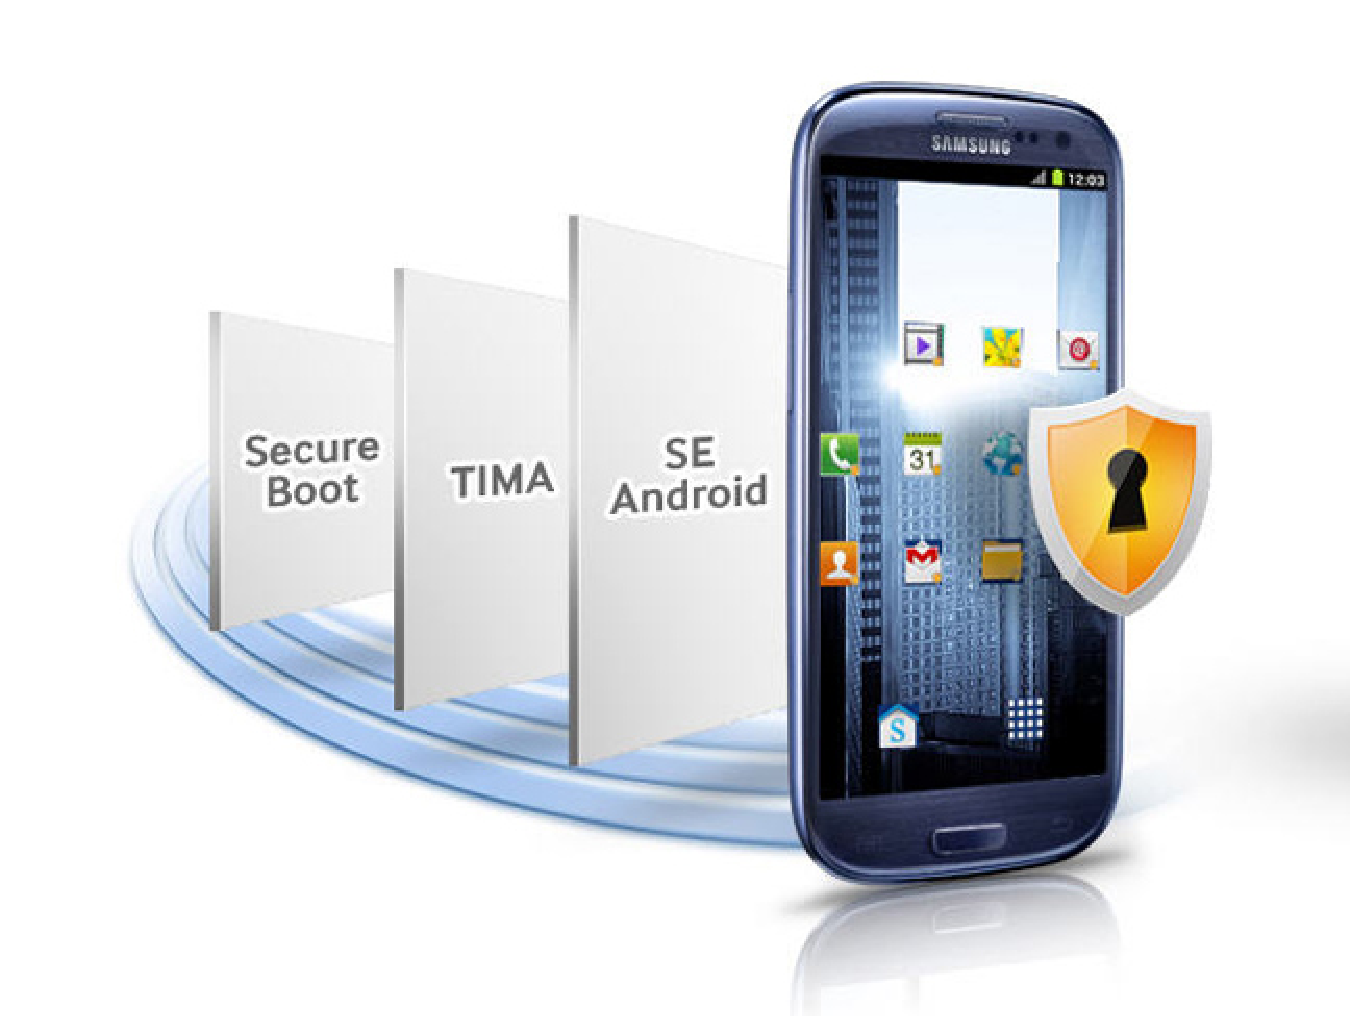
\includegraphics[scale=0.3]{img/samsung_knox_nueva.eps}
		\caption{Samsung's Knox utility architecture. Source: http://www.samsung.com/global/business/mobile/solution/security/samsung-knox}
	\label{fig:img_knox_01}
	\end{center}
\end{figure}

%----------------------------------------------------------------------------

\subsection{Good's Bring Your Own Device solution}
\label{subsec:goodsbyod}

Good Technology is a company that was founded in 1996 in California. The philosophy followed by Good is similar to Samsung's Knox one: to create a secure container that places an unreachable partition between personal and business data to protect company's assets. The solutions that they offer \cite{Good_tool} are similar than the previous ones. They have focused in mobile (not laptops) devices, though they support a number of OSs, and in separarting personal and company data. A Good's secure Network Operations Center (NOC) is introduced for dealing with the unauthorised devices, or providing access to secure collaboration solutions (email, PIM, calendar), intranet, and in-house or third-party mobile applications. Finally, Good offers best practice recommendations to help the company's BYOD policies such as reimbursements and stipends. There is a document available at Good's webpage\footnote{\url{http://www1.good.com/mobility-management-solutions/bring-your-own-device}} which contains several questions about Information Security Policies and how to cope them all.

%----------------------------------------------------------------------------

\subsection{BlackBerry Balance}
\label{subsec:blackberrybalance}

This security package was announced as a feature of BlackBerry 10 \cite{Blackberry_tool}. Nevertheless, it is available with BlackBerry Enterprise Service 10, which is a device management, security and app management for BlackBerry, iOS and Android devices. It is necessary to activate BlackBerry Balance for having available some security features, all related or similar to the aforementioned. For instance, as shown in Figure \ref{fig:blackberry_bal}, a message is displayed when the user tries to copy work data and then paste it into personal apps. Also, user attemptings for actions that are not permitted in the company ISP, or may cause secure work information to be in contact with personal applications, these actions won't be permitted. On the other side, employees are able to access information annd applications related to their personal lives, while staying connected to important work information when they need to perform. Finally, another known feature is also offered by Blackberry, so if the device gets lost or stolen, or if the employee leaves the organization, there will be an option to wipe just work information and it can be done remotely.

\begin{figure}
	\centering
		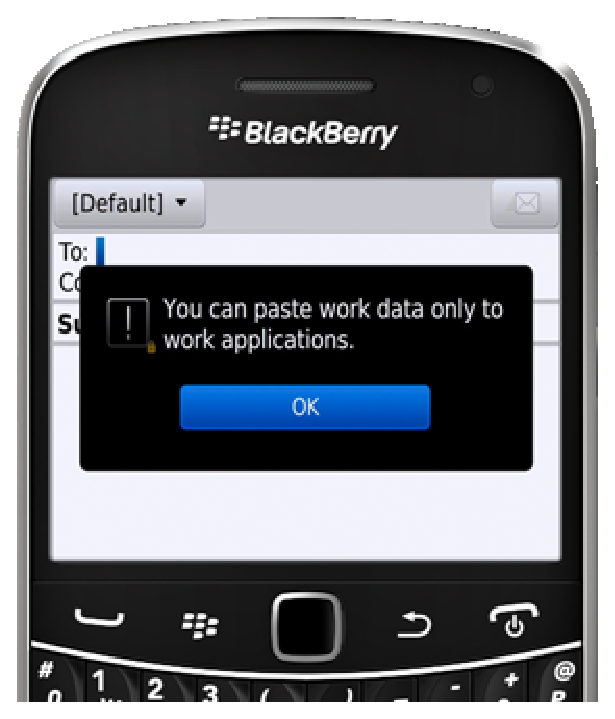
\includegraphics[scale=0.5]{img/Blackberry_balance.eps}
		\caption{Displayed message in new Blackberry 10 when attepmting to copy sensitive company data. Source: http://uk.blackberry.com/business/software/blackberry-balance.html.}
	\label{fig:blackberry_bal}
\end{figure}


%----------------------------------------------------------------------------
%%%%%%%%%%%%%%%%%%%%%%%%%%%%%%%%   MUSES %%%%%%%%%%%%%%%%%%%%%%%%%%%%%%%%%%%%
%----------------------------------------------------------------------------


\section{Multiplatform Usable Endpoint Security System}
\label{sec:muses}

MUSES system will work as presented in Figure \ref{fig:system_overview}. The user interacts with the devices, own or corporate, through the MUSES graphical interface and inside his or her own context (situation, connection, status). This application includes two modules, a \textit{controller} and an \textit{actuator}. The first one monitorizes the environment (context) and the user's behaviour, translating his/her actions into a sequence of events. These events, along with the patterns defining the user's conduct, are processed by the system in real-time by means of a Risk and Trust Analysis Engine (RT2AE) and an Event Correlation module. Then, a decision is taken in the corporate security operations centre (SOC) side, considering the RT2AE output and the set of security rules adapted to that specific user and context. The correspondent feedback is communicated to the user through the \textit{actuator}, which is also in charge of triggering the recommended actions to stop the user's or application's doings, in case it is required.

\begin{figure}
\centering
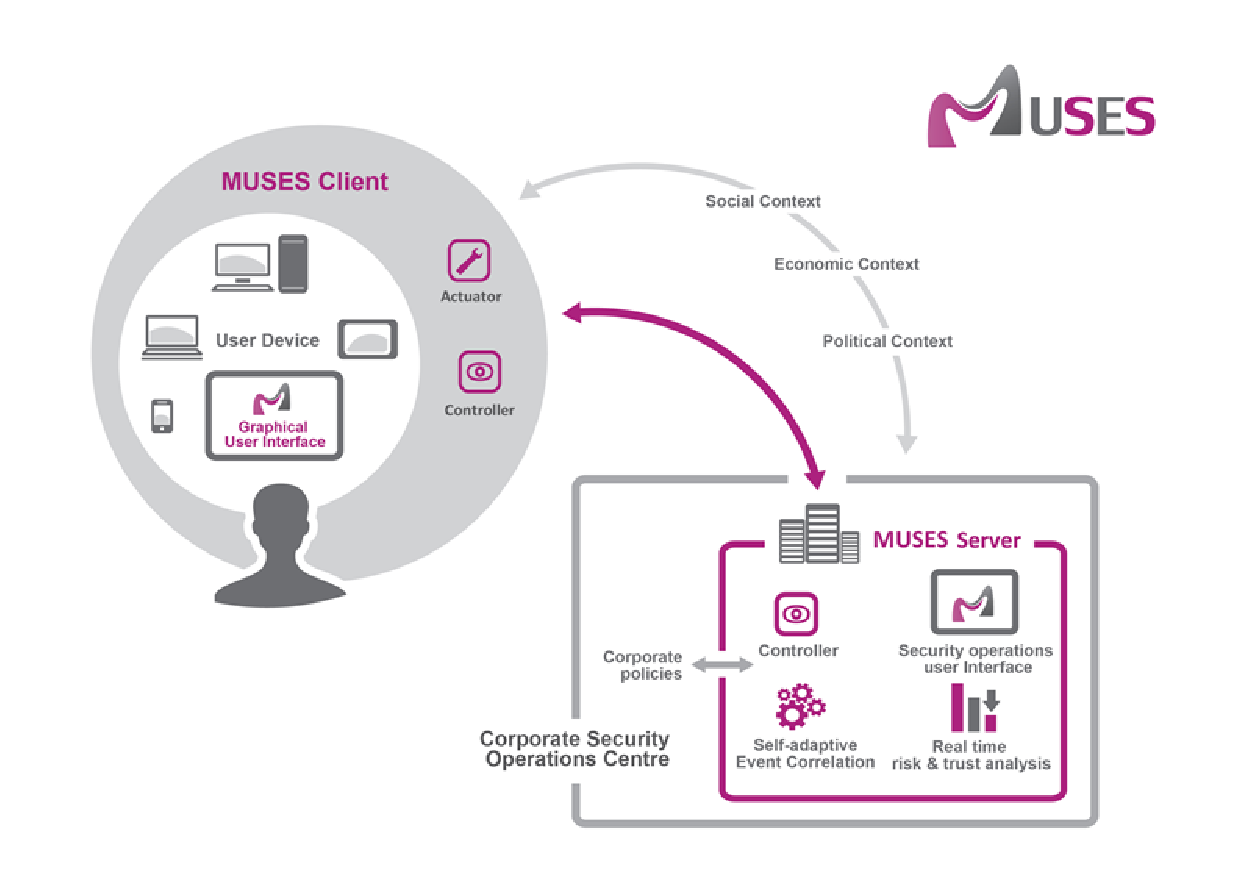
\includegraphics[scale=0.55]{img/system_overview.eps}
\caption{MUSES system overview.\label{fig:system_overview}}
\end{figure}

The system architecture can be seen in Figure \ref{fig:architecture}. It is a client-server approach in which the \textit{client} program will be installed in every user's device independently of the platform (operative system and type of device). This client contains a \textit{monitorization module}, which gathers the performed sequence of events and user context information; a \textit{controller module} in charge of take some light decisions considering the server response to the current situation (it will also take the control in case the device cannot connect with the server). The device controller will trigger the \textit{actuator} if necessary. This module will provide the user with some feedback, and will interact with the applications being monitorized if recommended or required.

The \textit{server} side would be installed in the corporate SOC. This application contains, in addition to an user interface to manage it, the main modules in the security-aimed decision process: the \textit{RT2AE} and the \textit{Event Correlator}. These components are connected between them and also with the main \textit{Controller}, that will connect with the device side sending the selected set of security rules that better fit with the current situation, along with the actions to be performed according to them.

\begin{figure}
\centering
\includegraphics[scale=0.45]{img/muses_architecture.eps}
\caption{Proposed architecture. Design art by S2 Grupo. http://www.s2grupo.es/. \label{fig:architecture}}
\end{figure}

One of the main features of the presented system is the self-adaptation (to the user and context) of the set of rules. To this aim, asynchronously to the system working, there will be run a process which will consider the whole amount of historic information regarding user's behaviour and context, and refine it by means of computational intelligence and machine learning techniques. Thus the set of security rules will be adapted to the every user in the system, updating some of the existent rules and creating new ones (always respecting the corporate security policies).
Moreover, some predictive models will be also obtained applying other soft computing techniques, so the user's potentially dangerous behaviour will be anticipated.


%MUSES (or Multiplatform Usable Endpoint Security) is a project co-funded by the European Commission under the Seventh Framework Programme. This MUSES project has concluded it first year (from a total of three) and is expected to develop a prototype (Prototype \#1) for Android Devices in the second year.
%The final product of MUSES for companies will be a system which will be installed in workers' devices and enterprise servers. There will be compiled versions of MUSES deployed on these kinds of devices:
%
%\begin{enumerate}
%	\item Portable devices. These are laptops that can be used in the company's premises or elsewhere.
%	\item Mobile devices. These include smartphones and tablets.
%	\item Enterprise servers.
%\end{enumerate}
%	
%The first two kinds can be owned either by the company itself or their employees (or their co-workers, where co-workers are indirect employees of the company; the term generally refers to the employees of contractor companies.).
%The very definition of MUSES as multiplatform usable endpoint security implies that the MUSES solution should be deployable and run on a number of platforms and operating systems. Being multiplatform is a key requirement for the adoption of MUSES as part of a wide range of corporate security strategies.
%
%In order to achieve its stated goals the MUSES system should be able to: capture user's behaviour, decide in real-time if user's behaviour poses a security threat, propose adaptations of the security policies based on patterns of user's behaviour, provide usable feedback to the user (based on security threat), and apply necessary adaptations and manipulation of context.

%----------------------------------------------------------------------------
%%%%%%%%%%%%%%%%%%%%%%%%%%%%%%%   COMPARISON  %%%%%%%%%%%%%%%%%%%%%%%%%%%%%%%
%----------------------------------------------------------------------------

\section{MUSES Advantages Against other Solutions}
\label{sec:comparison}


The main differences with MUSES, is that it will be also a free, open-source, platform independent solution. This is an important advantage because all the existent tools take into account only smartphones and tablets, but MUSES covers laptops and company PCs too. Moreover the companies need specific operative system and server (like Windows Server, for instance). Even more, for the case of Samsung Knox, companies must work with an specific (though they can choose from a list) MDM service for being able of deploy Knox in their environments. Other big plus of the MUSES system is its new feature of self-adaptiveness. MUSES is able to adapt to changes, either regarding corporate security policies, newly discovered vulnerabilities or threats, different environments of use or user profiles. 

In addition, the existing products are mostly policy-based, but MUSES takes its decisions not only considering policies, but also based on the terminals/users context (location, connected networks and so on), to really understand the real danger of a specific action.


%----------------------------------------------------------------------------
%%%%%%%%%%%%%%%%%%%%%%%%%%%%%%%   CONCLUSIONS  %%%%%%%%%%%%%%%%%%%%%%%%%%%%%%%
%----------------------------------------------------------------------------

\section{Conclusions}
\label{sec:conclusions}

In this work, there were presented many tools that prove how information security in the enterprise is adapting to this emergent philosophy of BYOD. For each one, the main features and working environments were detailed. Also it was shown, by the introduction to MUSES project, how the European Community is specially aware about that and is developing a free solution for managing employees privacy, and securing companies' assets in this changing environment. The paper has been written through a vast literature review; the tools were not possible to be tested because, in the first place, all of them but MUSES are neither free nor open source and, secondly, some of them has just been released, such as the Samsung Knox (release delayed from April/May to the end of 2013) or MUSES, which first prototype is still under development.

%%%%%%%%%%%%%%%%%%%%%%%%%%%%%  ACKNOWLEDGEMENTS %%%%%%%%%%%%%%%%%%%%%%%%%%%%%%%%

\section{Acknowledgements}
This work has been supported by MUSES FP7 project, and in part by the P08-TIC-03903 project awarded by the Andalusian Regional Government, the FPU Grant 2009-2942, and the TIN2011-28627-C04-02 project, awarded by the Spanish Ministry of Science and Innovation.

\bibliographystyle{elsarticle-num}

% Antonio - Poner la bibliograf�a en fichero .bib

\begin{thebibliography}{00}

%\bibitem{ids13}
%Sommestad T., Hunstad A.. \emph{Intrusion detection and the role of the system administrator.}, from Swedish Defence Research Agency (FOI), Link�ping, Sweden, 2013.

%\bibitem{m2m12}
%NTT DOCOMO, \emph{DOCOMO to Launch Global M2M Platform}, in M2M Magazine, December 2012.
%http://www.machinetomachinemagazine.com/2012/12/05/docomo-to-launch-global-m2m-platform/.

%\bibitem{suites12}
%The Radicati Group Inc., report \emph{Microsoft Office 365 - Analysis and Forecast, 2012-2016}. June 2012. 

\bibitem{Adams_Users05}
A.~Adams and A.~Sasse.
\newblock {\em Users are not the enemy}.
\newblock Security and Usability: Designing Systems That People Can Use.
  O\'Reilly Associations, 2005.

\bibitem{SecPolComp12}
Al-Omari, A., El-Gayar, O., Deokar, A., and Walters, J. \emph{Security Policy Compliance: User Acceptance Perspective}. 45th Hawaii International
Conference on System Sciences (pp. 3317-3326). IEEE, 2012.

\bibitem{BYOD13}
Bacik, Sandy, \emph{Security Implications of Bring Your Own Device, IT Consumerization, and Managing User Choices}, in Information Security Management Handbook, Sixth Edition, Volume 7, pp. 133-142, 2013.

\bibitem{Blackberry_tool}
Blackberry.
\newblock Blackberry balance.
\newblock http://es.blackberry.com/business/software/blackberry-balance.html.

\bibitem{SecPolComp10}
Bulgurcu, B., Cavusoglu, H., and Benbasat, I. \emph{Information security policy compliance: an empirical study of rationality-based beliefs and information security awareness}. MIS Quarterly, 34(3), 523�548. 2010.

\bibitem{SecPol09}
Charles Cresson Wood and Dave Lineman. \emph{Information Security Policies Made Easy Version 11}. Information Shield, Inc. 2009.

\bibitem{android11}
Clemens Orthacker, Peter Teufl, Stefan Kraxberger, G�nther Lackner, Michael Gissing, Alexander Marsalek, Johannes Leibetseder, and Oliver Prevenhueber. \emph{Android Security Permissions � Can We Trust Them?}. MobiSec Session on Smartphone Security, Aalborg 2011.

\bibitem{Good_tool}
Good's Technology.
\newblock BYOD Solution.
\newblock
  http://www1.good.com/secure-mobility-solution/bring-your-own-device.html.
	
\bibitem{IBM_tool}
IBM.
\newblock Hosted mobile device security management.
\newblock
  http://www-935.ibm.com/services/us/en/it-services/managed-security-services-cloud-computing-hosted-mobile-device-security-management.html.
	
\bibitem{ibm11}
I-Lung Kao, \emph{IBM Security Services. Securing mobile devices in the business environment}, IBM, 2011.

\bibitem{Schu_SecPatterns05}
M.~Schumacher, E.~Fernandez-Buglioni, D.~Hybertson, F.~Buschmann, and
  P.~Sommerlad.
\newblock {\em Security Patterns: Integrating Security and Systems
  Engineering}.
\newblock John Wiley \& sons, 2005.

\bibitem{SecPolComp07}
M. Siponen, S. Pahnila, and A. Mahmood. \emph{Employees� adherence to information security policies: an empirical study}. In IFIP International Federation for Information Processing, Volume 232, New Approaches for Security, Privacy and Trust in Complex Environments pp. 133-144, 2007.

\bibitem{MIT05}
R.P. Lippmann, K.W. Ingols, C. Scott, K. Piwowarski, K.J. Kratkiewicz, M. Artz, and R.K. Cunningham. \emph{Evaluating and Strengthening Enterprise
Network Security Using Attack Graphs}. Project Report IA-2. Lincoln Laboratory, Massachusetts Institute of Technology, October 2005.

\bibitem{Opp_Security11}
R.~Oppliger.
\newblock Security and privacy in an online world.
\newblock {\em IEEE Computer}, 44(9):21--22, September 2011.

\bibitem{SecPolComp09}
R. S. Shaw, C. C. Chen, A. L. Harris, and H.-J. Huang. \emph{The impact of information richness on information security 
awareness training effectiveness}. Computers \& Education, vol. 52, pp. 92-100, 2009.

\bibitem{Samsung_tool}
Samsung KNOX.
\newblock
  https://www.samsungknox.com.
	
\bibitem{Sophos_tool}
Sophos.
\newblock Mobile control.
\newblock http://www.sophos.com/en-us/products/mobile-control.aspx.

\bibitem{SecPolPenalty09}
T. Herath and H. R. Rao. \emph{Protection motivation and deterrence: a framework for security policy compliance in organisations}. European Journal of Information Systems, vol. 18, pp. 106-125, 2009.


%Para fijarme
%\bibitem{GAs_Goldberg89}
%Goldberg D.E., Korb B., Deb K., \emph{Messy genetic algorithms: motivation, analysis, and first results}, Complex Systems, 3(5), pp. 493--530, 1989.


\end{thebibliography}

\end{document}
